\chapter{Hierarchical Clustering}
\label{ch:hierarchical_clustering}

\newthought{We are interested in finding clusters in our data}. That is, we would like to identify groups of data instances that are close together, similar to each other. Consider a simple, two-featured data set (see the side note) and plot it in the \widget{Scatter Plot}. How many clusters do we have? What defines a cluster? Which data instances should belong to the same cluster? How does the clustering algorithm actually work?

\begin{marginfigure}
    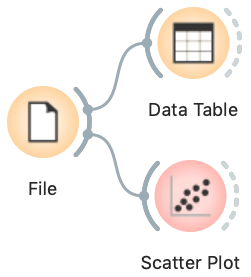
\includegraphics[scale=0.4]{workflow_scatterplot.png}
    \caption{We will introduce clustering with a simple data set on students and their grades in English and Algebra.
Load the data set from \url{http://file.biolab.si/text/grades.tab}.}
\end{marginfigure}

First, we need to define what we mean by "similar". We will assume that all our data instances are described (profiled) with continuous features. One simple measure of similarity is the Euclidean distance. So, we would like to group data instances with small Euclidean distances.

\begin{figure*}[h]
    \vspace{1cm}
    \centering
    \infinitewidthbox{
    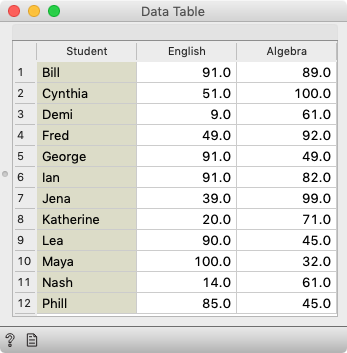
\includegraphics[scale=0.4]{grades_table.png}
    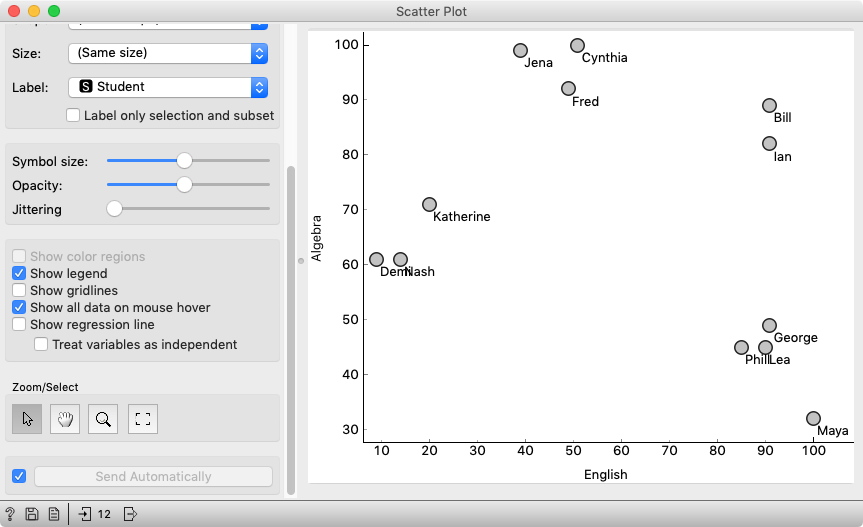
\includegraphics[scale=0.4]{grades_scatterplot.png}
    }
    \caption{There are different ways to measure the similarity between clusters. The estimate we have described is called average linkage. We could also estimate the distance through the two closest points in each clusters (single linkage), or through the two points that are furthest away (complete linkage).}
\end{figure*}

Next, we need to define a clustering algorithm. Say that we start with each data instance being its own cluster, and then, at each step, we join the clusters that are closest together. We estimate the distance between the clusters with, say, the average distance between all their pairs of data points. This algorithm is called hierarchical clustering.

\clearpage

One possible way to observe the results of clustering on our small data set with grades is with the following workflow:

\begin{marginfigure}
    \centering
    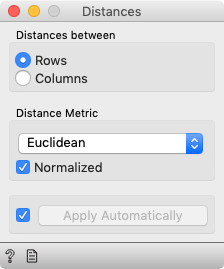
\includegraphics[scale=0.6]{distances.png}
\end{marginfigure}

\begin{figure}[h]
    \centering
    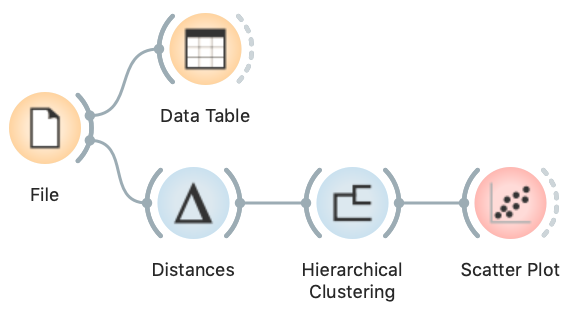
\includegraphics[scale=0.4]{workflow_clustering.png}
    \caption{$\;$} % empty caption for proper pagesetting
\end{figure}

Couldn’t be simpler. Load the data, measure the distances, use them in hierarchical clustering, and visualize the results in a scatter plot. The \widget{Hierarchical Clustering} widget allows us to cut the hierarchy at a certain distance score and output the corresponding clusters:

\begin{figure*}[h]
    \centering
    \newcommand{\clustering}{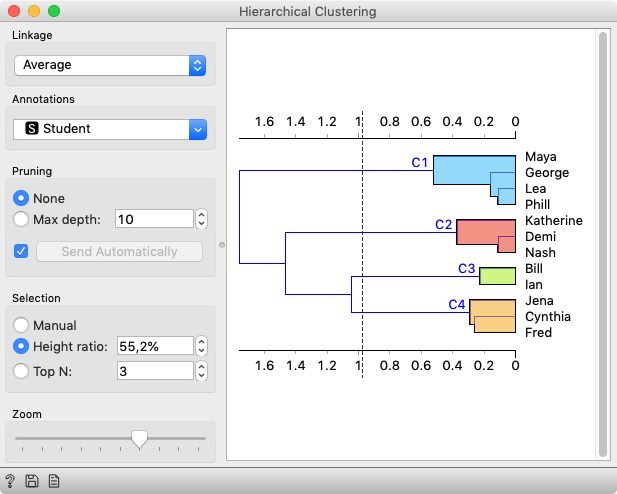
\includegraphics[scale=0.4]{hierarchical_clustering.png}}
    \newcommand{\plot}{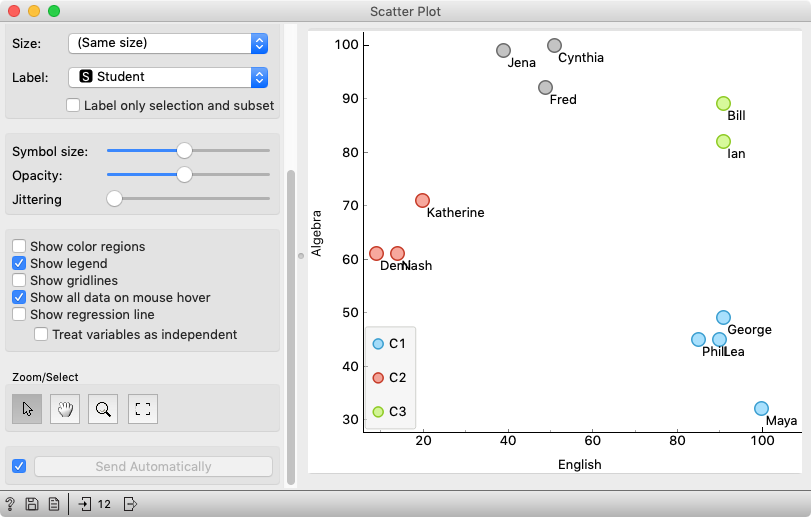
\includegraphics[scale=0.4]{scatterplot_clustered.png}}
    \infinitewidthbox{
    \stackinset{r}{-0.5\linewidth}{t}{+0.3\linewidth}{\plot}{\clustering}\hspace{8cm}
    }
\end{figure*}
